\documentclass[11pt,a4paper]{article} 


\setcounter{secnumdepth}{3}
\usepackage[T1]{fontenc}
\usepackage[utf8]{inputenc}
\usepackage{lmodern}
\usepackage{pdflscape}
\usepackage{lipsum}
\usepackage{graphicx}
\usepackage{caption}
\usepackage[font=footnotesize]{caption}
\usepackage{apacite}
\usepackage{color}
\usepackage{amsmath}
\usepackage[margin=1.5in]{geometry}
\usepackage{booktabs} 
\usepackage{xcolor}
\usepackage{float}
\usepackage{array}
\usepackage{setspace}
\usepackage{gensymb}
\usepackage{subcaption}
	\doublespacing

\date{}
\title{\huge{}}

\graphicspath{{./AE_Teapot}} 

\begin{document}
\maketitle


\section{Introduction} 

In Chapter \ref{AE_LSA}, we conducted two experiments to probe the robustness of the attraction effect with complex, naturalistic stimuli. This research question arose from the debate on the real-world relevance of the attraction effect, which started with the study of \citeA{Frederick2014} describing numerous failed replication attempts where the choice options were naturalistic objects. They drew the conclusion that the attraction effect is only present in choice settings where the options have numerical attributes. The findings from our experiments confirmed \citeauthor{Frederick2014}'s results in that we have not found any evidence for the attraction effect using movies posters as naturalistic stimuli.

However, as discussed in Chapter  \ref{AE_LSA}, there is substantial evidence that the attraction effect is \textit{not} restricted to choice settings where the options have numerical attributes. In value-based decision making, \citeA{Farmer2017} have demonstrated the attraction effect using perceptual representation of gambles. In one version, they adopted the rectangle stimuli of \citeA{Trueblood2013} to represent the probability and the nominal amount to be won (therefore, the area of each rectangle corresponded to the expected value of the gamble). In another experiment, the probability of the gamble was represented by the proportion of randomly distributed coloured squares in a 10x10 grid, whereas the nominal amount was represented as the proportion of coloured squares in another 10x10 grid. 

While these perceptual tasks are clear departures from the commonly used numerical attributes format, they are still very similar to it in one respect. Specifically, in both versions, the two attribute dimensions are spatially separated, and thus can be attended independently. We argue that independent processing of attribute dimensions can be key in explaining why the attraction effect is so elusive in some choice contexts. To design an experiment that tests this hypothesis, we draw on insights from decades of research on the perception and processing of multiattribute stimuli.

\subsection{Integral and separate dimensions} 

The idea that multiattribute stimuli can be classified based on the perceived separability of the attribute dimensions first arose from research focusing on similarity judgements using the method of multidimensional scaling (MDS; \citeNP{Kruskal1964}; \citeNP{Shepard1980}). In essence, MDS can be used to build a low-dimensional geometrical representation of the perceived similarity between pairs of objects \cite{Hout2013}. In this representation, the objects are points in a Cartesian coordinate system, and the distance between them corresponds to their perceived similarity (so that more similar objects are closer to each other). This distance can be calculated in various ways, of which the Euclidean distance metric, $\delta = \sqrt{\delta_x^2 + \delta_y^2} $ is the most intuitive and well-known, and was consequently used in the first applications of MDS to similarity judgements.

However, \citeA{Attneave1950} challenged the appropriacy of the Euclidean distance metric. He proposed that an alternative distance measure, the city-block metric, $\delta = \delta_x + \delta_y $ provides a much better fit for the similarity judgement data he collected in his experiments, where he asked participants to make similarity judgments between parallelograms, squares and triangles with varying dimensions, including size, tilt, and colour. According to the city-block metric, the perceived overall distance is simply the sum of the distances along the attribute dimensions.  

In contrast with \citeauthor{Attneave1950}'s results, \citeA{Torgerson1958} have found strong support for the Euclidean metric in an experiment where participants were asked to provide similarity judgements for Munsell colour chips that differed in brightness and saturation. These contradictory results led researchers to examine how the perceived similarity of two objects depend on their attribute characteristics. 

In fact, the Euclidean and city-block distance metrics reflect two fundamentally different ways of perceiving object similarity. In particular, the Euclidean distance metric is invariant to axis rotation, while the city-block metric is not. This means that objects whose pairwise similarity can be best described by the city-block metric have ``privileged'' psychological dimensions, whereas the Euclidean metric is more appropriate for objects that are processed ``holistically'', where the underlying attribute dimensions may not even be perceived separately \cite{Shepp1989}. 

\citeA{Shepard1964} argued that these differences can be explored by analysing how participants justify their similarity judgements for these two classes of stimuli. For example, when the attributes can be perceived independently (stimuli that he called \textit{analyzable}), participants have almost always referred to the distinct attribute dimensions when describing differences. However, when the stimuli is processed holistically (for dimensions he called \textit{unitary}), participants tended to describe the difference along one, ``combined'' dimension, indicating that the two attribute dimensions cannot be perceived separately (and that the participant might not even be aware that there are multiple underlying dimensions). 

\citeA{Lockhead1966} investigated how the effect of dimensional redundancy differs for stimuli with \textit{separable} and \textit{integral} dimensions (these are the respective equivalents of \textit{analyzable} and \textit{unitary} in \citeauthor{Shepard1964}'s terminology). A redundancy gain is said to occur when performance in a selective attention task (most typically discrimination, detection, or categorization) is improved (faster and/or more accurate responses) when the two attribute dimensions vary in a correlated manner. Previous research have found redundancy gains for integral dimensions (Munsell color chips; \citeNP{EriksenHake1955}) but not for separable dimensions (visual positions of X's and O's; \citeNP{GarnerLee1962}). \citeauthor{Lockhead1966} argued that the redundancy gain occurs because integral attributes cannot be attended separately, and that the concept of redundancy gain should be key in the definition of integral attribute dimensions. 

Drawing on  \citeauthor{Lockhead1966}'s findings, \citeA{GarnerFelfoldy1970} demonstrated that integral dimensions give rise to redundancy gains and interference effects within the same experimental task. Interference effects  (slower and less accurate responses) can be observed if the two integral dimensions are orthogonal (vary in an uncorrelated manner). They proposed a new definition for integral attribute dimensions. According to this, dimensional integrality (1) can be best described by an Euclidean distance metric, (2) produces redundancy gains if the dimensions vary in a correlated fashion, and (3) results in interference effects when the two dimensions are orthogonal. The experimental paradigm where these assumptions can be tested with a control, correlated, and filtering condition has later became known as the Garner interference task \cite{Burns2014}.

More recent research have focused on how the processing of stimuli with integral and separable dimensions differ in perceptual categorization tasks. These studies have typically analysed reaction times and choice probabilities in sequential sampling modelling frameworks. \citeA{Little2011} investigated whether the processing of multiattribute stimuli depends on the spatial separability of the attribute dimensions. They found that when the attribute dimensions are spatially separated (e.g., the base width of a lamp and the curvature of its top piece), they are processed in a sequential, serial manner. However, when the attribute dimensions are spatially overlapping, such that both attributes can be attended simultaneously (e.g., the colour of a rectangle and the position of an inset bar), a mixture of serial and parallel processing of dimensions occur. In a follow-up study, they found strong evidence that stimuli with integral attributes (e.g., brightness and saturation) are processed in a coactive fashion, where the attribute information is combined into a single processing channel \cite{Littleetal2013}, as opposed to the parallel and serial model, where there the are two independent accumulation processes for the two attribute dimensions.

While caution is warranted when applying insights from perceptual categorization to value-based decision making due to the inherent differences between the two choice tasks, if object processing share commonalities in the two contexts, it bears significance for any research that aims to investigate the cognitive mechanism underlying the attraction effect in preferential choice.   Crucially, most sequential sampling models that are able to accommodate the attraction effect rely on the assumption of attribute-wise processing of choice options. In addition, eye-tracking evidence suggests that single-attribute pairwise comparisons play a key role in the attraction effect \cite{Noguchi2014}.

To elucidate whether it is the separable nature of the choice options that give rise to the attraction effect in value-based decision making, we conducted an experiment to test whether the strength of the effect depends on stimuli presentation. Participants were first taught a valuation rule in the learning stage, and then were instructed to use this rule in the choice stage to identify the most valuable option from attraction-type choice triplets created form two kinds of artificial stimuli (separable and integral version). 

\section{Experiment 1} 


\subsection{Method}

In this experiment, our aim was to investigate the hypothesis that the strength of the attraction effect depends on the separability of the attribute dimensions. To this end, we created two versions of the same stimuli: a ``traditional'' version, where the two attribute dimensions have numerical values (numerical condition), and a perceptual version, where the attribute dimensions are integral, and thus cannot be attended independently (pictorial condition). We expected to see the attraction effect in the numerical condition, where the options can be compared along an attribute dimension, but not in the pictorial condition, where the options can only be processed holistically.

Designing a value-based choice experiment where the attribute dimensions are integral and preferences are monotone and continuous is challenging. To be consistent with previous research, we chose the most well-known integral stimuli in the literature, Munsell colors with a fixed hue, but varying brightness and intensity. Numerous studies have established that these attribute dimensions are integral, and therefore are processed holistically (e.g., \citeNP{EriksenHake1955}; \citeNP{GarnerFelfoldy1970}). 

We are only aware of a few studies that used perceptual stimuli in a preferential choice context. In these, the options' value naturally depended on the perceptual representation of the attribute dimensions (e.g., height and width of rectangle, where the value is given by the area;  \citeNP{Trueblood2013}). However, when the attributes are integral, it is much harder to ``induce'' preferences based on a valuation rule, due to the very nature of the stimuli (i.e, the inaccessibility of the independent dimensions). To overcome this difficulty, we first established a valuation rule that assigns a nominal value to each option, based on the two attribute dimensions. Participants had to learn this valuation rule in a learning stage that preceded the choice stage. They were then instructed to use the valuation rule when making decisions in the choice stage. While inducing preferences through the learning stage is somewhat artifical, this method ensured that participants had continuous, monotone and homogeneous preferences over our stimuli set. 

\subsection{Stimuli}

In colour theory, there are various ways to describe colours, of which the red-green-blue (RGB) colour model is perhaps the most well-known \cite{Colourtheory}. We created our stimuli using the hue-saturation-value (HSV) colour model. We will refer to saturation as intensity, and to value as brightness. In the HSV model, hue corresponds to the pure colour component of a colour, and is measured as the angle around the colour wheel, ranging from 0\degree\ to 360\degree, with cyan at 180\degree, and red at both ends of the wheel. For this entire experiment, we fixed the value of hue at 300\degree, resulting in a purple colour at the mean values of intensity and brightness. Intensity and brightness both vary between 0 and 1. As shown by Figure \ref{fig:explaincircle}, if brightness is set to 0.5, and hue is fixed at 300\degree, an intensity level of 0.1 corresponds to a completely grey colour, whereas a value of 0.9 results in an intense purple colour. Equally, it intensity is set at 0.5, and hue is fixed at 300\degree, a brightness level of 0.1 corresponds to a completely black colour, whereas a value of 0.9 results in a light purple colour.

\begin{figure}
\centering
\caption{Illustration of the intensity-brightness dimensions with hue fixed at 300\degree}
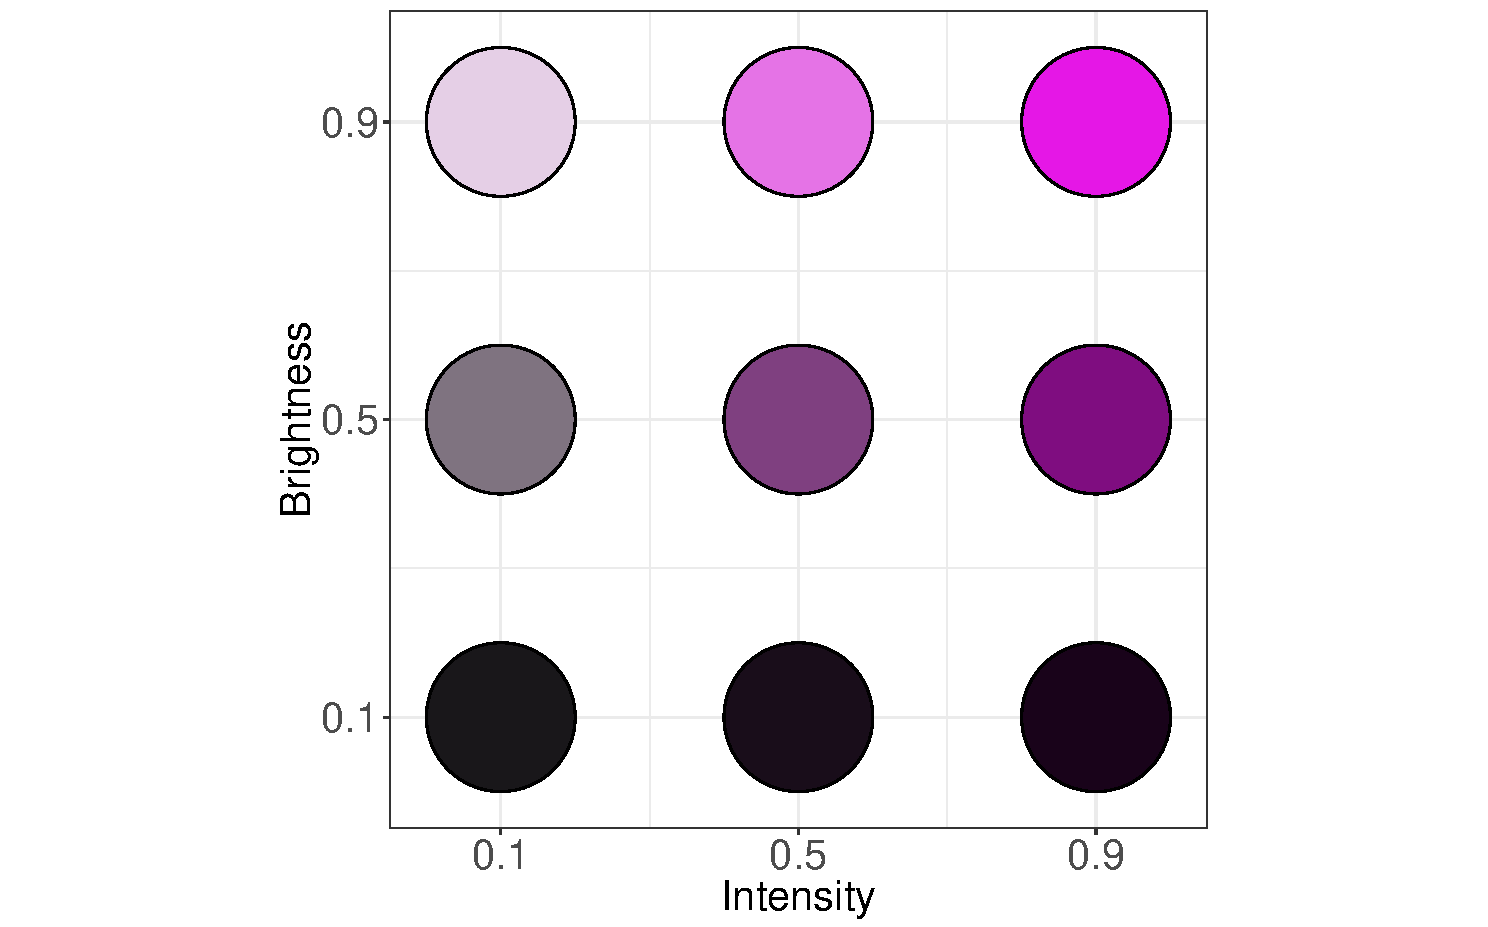
\includegraphics[width=1\textwidth]{./AE_teapots_Figure_1circles.pdf}
\label{fig:explaincircle}
\end{figure}

Our stimuli were teapots with varying brightness and intensity levels. Participants were told that the levels of these two attributes determined each teapot's value. In the numerical condition, the brightness and intensity values were displayed numerically, whereas in the pictorial condition, it was the colour of the teapot that determined the value (this was generated with varying brightness and intensity levels that determined the teapot's value, just like in the numerical condition).  

\subsubsection{Choice triplet selection process}

Previous research has shown that one unit change in brightness is perceptually equivalent to a two unit change in intensity \cite{Newhall1940}, and we took this into account when constructing the rule that determines the value of each option, based on its brightness and intensity values. This relationship is captured by the the red line on Figure \ref{fig:explain}, which is defined by the equation
\begin{equation} \label{eq:redline}
 Brightness = 0.5 \cdot Intensity+ 0.25.
\end{equation}


All stimuli were required to fall within the boundaries of the black polygon displayed on Figure \ref{fig:explain}. The shape of the polygon ensured that intensity and brightness were restricted to fall between 0.05 and 0.95 and 0.15 and 0.85, respectively. This was necessary to avoid extreme attribute values that hinders the perception of the other attribute dimension (e.g., a very low brightness would translate into a black colour, regardless of the intensity value). To create an attraction effect choice triplet, we first determined the position of the target and competitor options within the polygon, followed by the decoy. Then, we calculated the nominal value of each of the three options using Equation \ref{eq:redline}, such that options that scored higher on the intensity and brightness attribute dimensions were assigned a higher nominal value.

\begin{figure}
\centering
\caption{Illustration of the choice triplet selection process.}
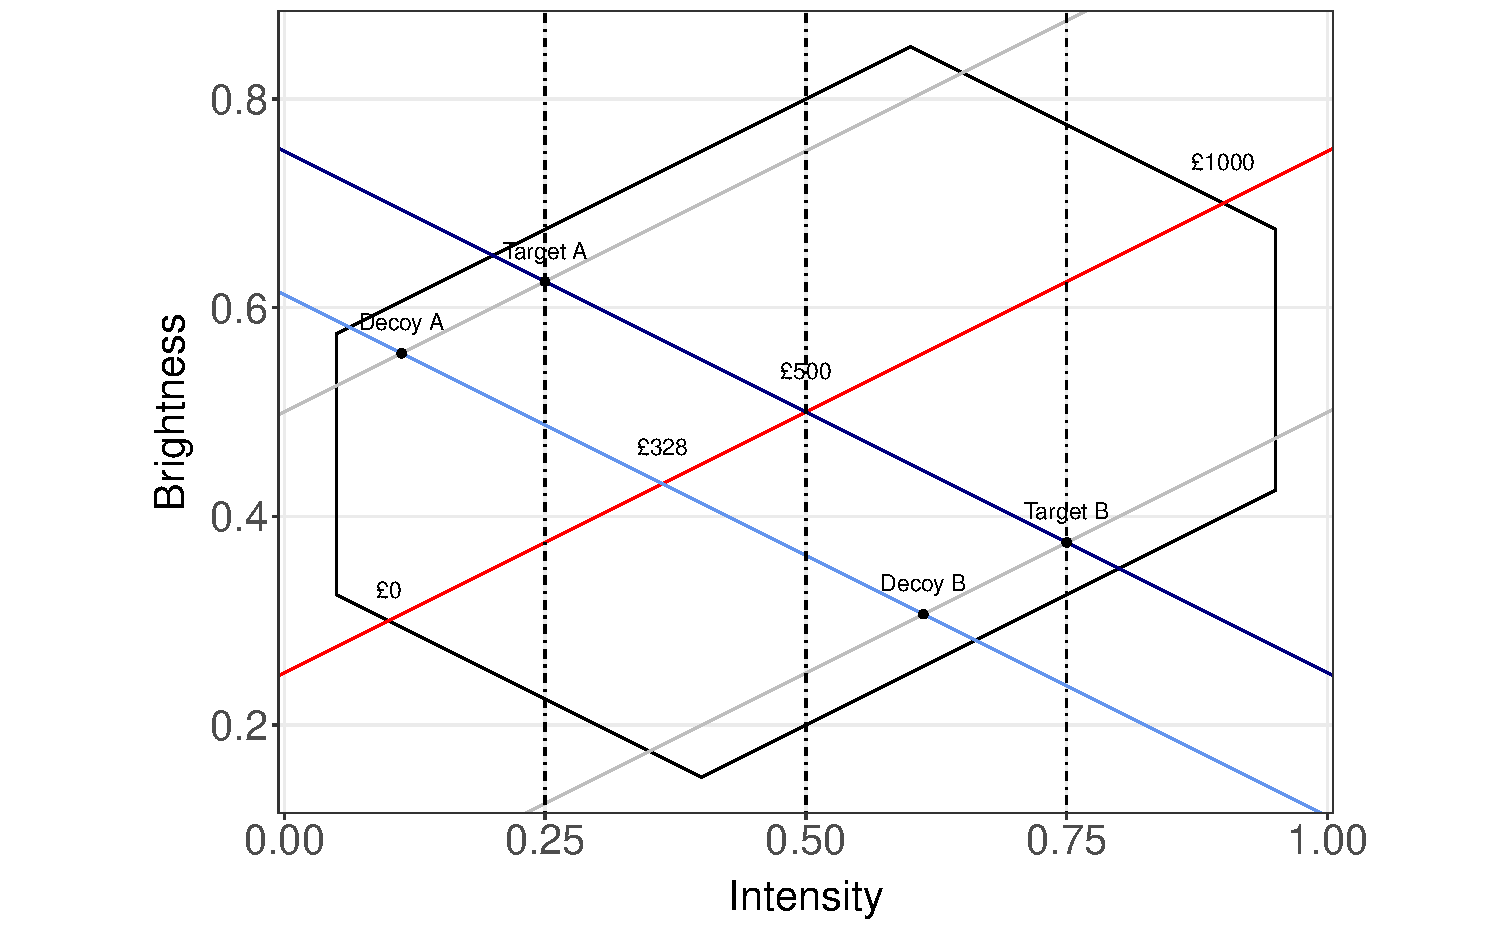
\includegraphics[width=1\textwidth]{./AE_teapots_Figure_1poly.pdf}
\label{fig:explain}
\end{figure}

 First, we determined the location of the target and competitor options. To do this, we first chose a random constant that was substituted into the following equation:
\begin{equation} \label{eq:blueline}
 Brightness = -0.5 \cdot Intensity + constant.
\end{equation}

In Figure \ref{fig:explain}, the dark blue line is defined by this equation, with $constant = 0.75$. The constant in Equation \ref{eq:blueline} was always chosen to ensure that the point where the red and blue lines cross fell within the polygon. On Figure \ref{fig:explain}, this is the center of the polygon where $Intensity = 0.5$ and $Brightness = 0.5$, and the dark blue line is thus the reflection of the red line over a vertical line defined by $Intensity = 0.5$ (the middle dashed line on Figure \ref{fig:explain}).




 We then created the two target candidates by selecting two points along the reflected line (the dark blue line), one in the upper half of the polygon (target candidate A), and another in the lower half (target candidate B), such that the distance between the two points had to be at least half the overall length of the dark blue line within the polygon. This was important in order to ensure that one of the target candidates has a high intensity and a low brightness value and vice versa, so that they will be perceived as markedly different by the decision maker (as is required from the target and the competitor in an attraction effect choice scenario). Having created the two target candidates, the next step in creating the choice triplets was to determine the position of the decoy option. 

To create the decoy, we first randomly decided which target candidate will be assigned a decoy option (Target A or Target B on Figure \ref{fig:explain}). We then again reflected the dark blue line through a vertical line that crossed the chosen target option (the dashed lines defined by $Intensity = 0.25$ and $Intensity = 0.75$ for Target A and Target B, respectively), which, depending on which target candidate was chosen to be the target, gave us one of the grey lines, which is parallel to the original red line. Naturally, any option along this line that lies to the left of the target will have a lower intensity and brightness value, and therefore will be inferior to it. 

However, all decoys need to satisfy two criteria. First, a decoy needs to be sufficiently far away from the target option, so that the dominance relationship can be easily identified. Perceiving the dominance relationship is especially problematic with naturalistic stimuli (as opposed to a choice scenario with numerical attributes where it can be identified with absolute certainty -- provided that the decision maker pays attention to the task). Therefore, we considered this criterion as the most important when creating the decoys. Second, a decoy cannot be too far away from the target, as they need to be somewhat similar to invoke an attraction effect choice situation.

Taking these considerations into account, we decided that the decoy's position should depend on the distance between the target and the competitor (as this can vary to an extent). This avoids situations where the decoy is also dominated by the competitor (this can happen if the target and the competitor are relatively close, while the target and the decoy are relatively far away from each other). Specifically, we decided that the distance between the target and the decoy along the brightness dimension (y axis) should be the 27.5\% of the overall difference between the target and the competitor along the same axis. This criterion uniquely defines a point along the grey line (either Decoy A or Decoy B in Figure \ref{fig:explain}).

Once we have decided on the exact brightness and intensity values for the attraction effect choice triplet, the next step was to determine the nominal value of the options. We assigned a nominal value to every point along the red line, starting with £0 and going up to £1000 (in the bottom left and top right corner in Figure \ref{fig:explain}, respectively, where the line crosses the polygon boundaries), so that any line parallel to the dark blue line is essentially a contour line, corresponding to a certain nominal value. Using these contour lines, we can assign a nominal value to any point within the polygon.

For example, as the dark blue line crosses the red line at exactly halfway through its length within the polygon, the target and competitor were assigned a value of £500. Then, once we calculated the position of the decoy, we were able to define the relevant contour line (light blue line in Figure \ref{fig:explain}), which corresponds to a nominal value of £328. 

\begin{figure}[!htb]
\centering
\caption{The 500 choice triplets that were used in the experiment.}
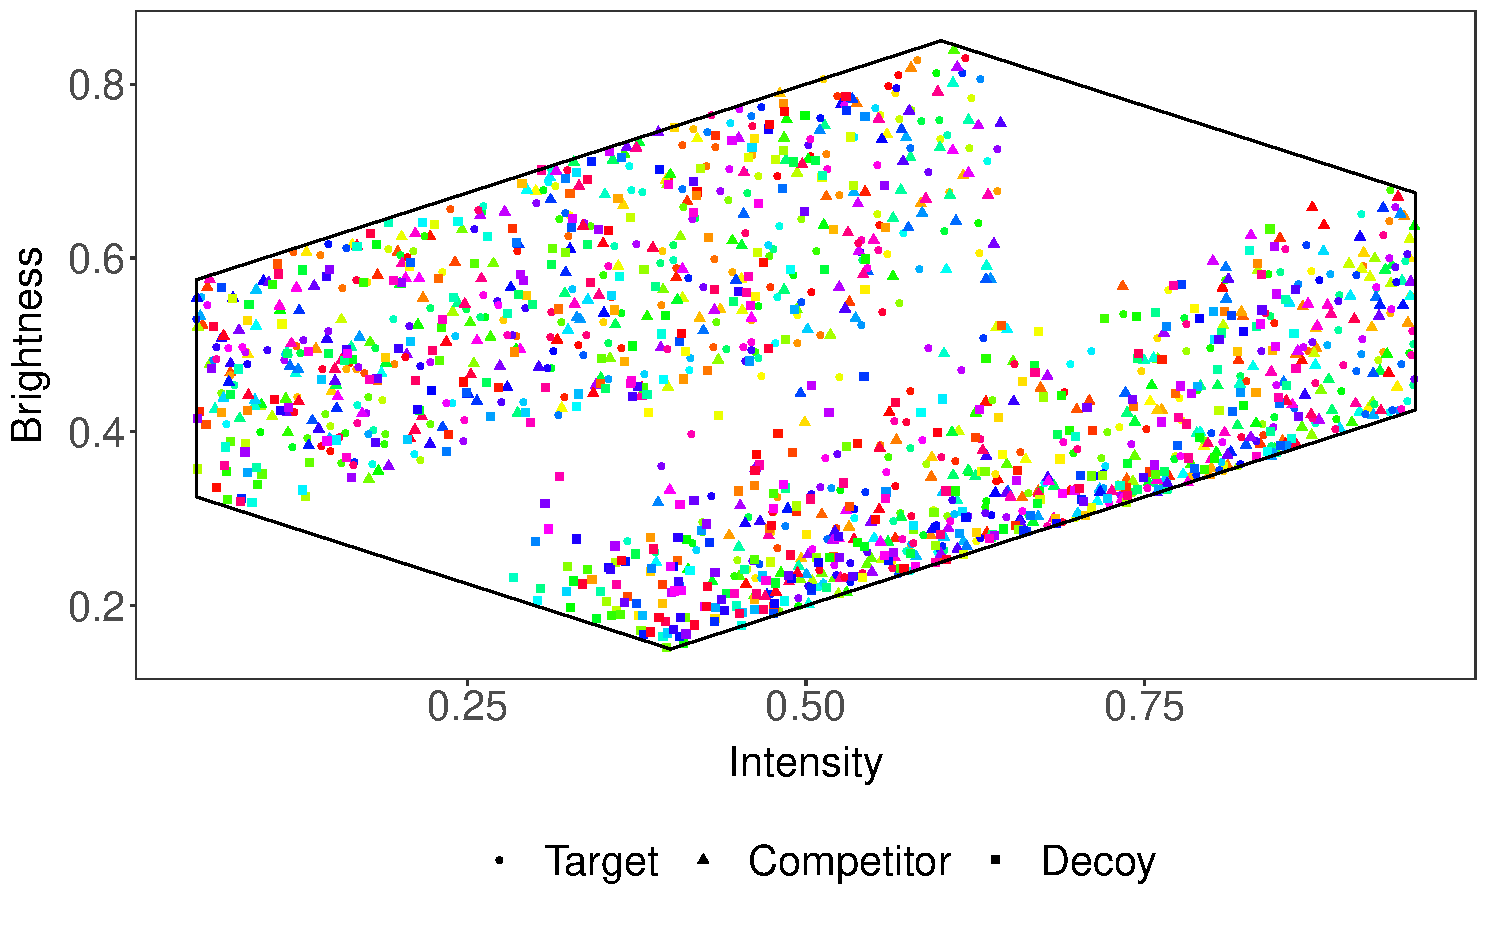
\includegraphics[width=1\textwidth]{./AE_teapots_Figure_2poly.pdf}
\label{fig:choice_sets}
\end{figure}

Using the method described above, we generated 500 choice triplets with target, competitor and decoy, as shown on Figure \ref{fig:choice_sets}, where each option is defined by its brightness, intensity and nominal value. In the pictorial condition, participants were presented coloured teapots, where the colour of each teapot was defined by the corresponding intensity and brightness value, and we instructed them to select the teapot with the highest nominal value. We hypothesised that using integer numbers will make comparisons cognitively less demanding in the numerical condition, therefore we transformed the raw brightness and intensity values by subtracting the minimum and multiplying them by 200. The raw intensity and brightness values fell between 0.05 and 0.95 and 0.15 and 0.85, and the new range of intensity and brightness values fell between 0 and 200 and 0 and 140, respectively.




\subsubsection{Experimental procedure}

The experiment consisted of a numerical and pictorial condition, each with two stages: a learning and a choice stage, which was the main task.  All participants were required to complete both conditions, and the order of the two conditions was determined randomly. 


The learning stage served to ``teach''  participants how to infer the nominal value of the options based on the numeric attributes/colour of the teapots. While a one-dimensional valuation rule can be fairly intuitive (e.g., the brighter or more intense the colour, the better) and thus easy to learn, when it comes to a two-dimensional learning rule, the interactions between the two integral dimensions can complicate the valuation process. For this reason, the choice stage in each condition was only accessible upon passing the corresponding learning stage. Before the learning stage, participants  were provided with a ``valuation map'', which served to explain how the nominal value depended on the attribute values (see Figure \ref{fig:valuemaps}). The example stimuli on the valuation maps were derived from four equally spaced contour lines, like the blue lines on Figure \ref{fig:explain}.


\begin{figure}[htp]
\centering
\caption{Value maps for both choice tasks in the experiment.}
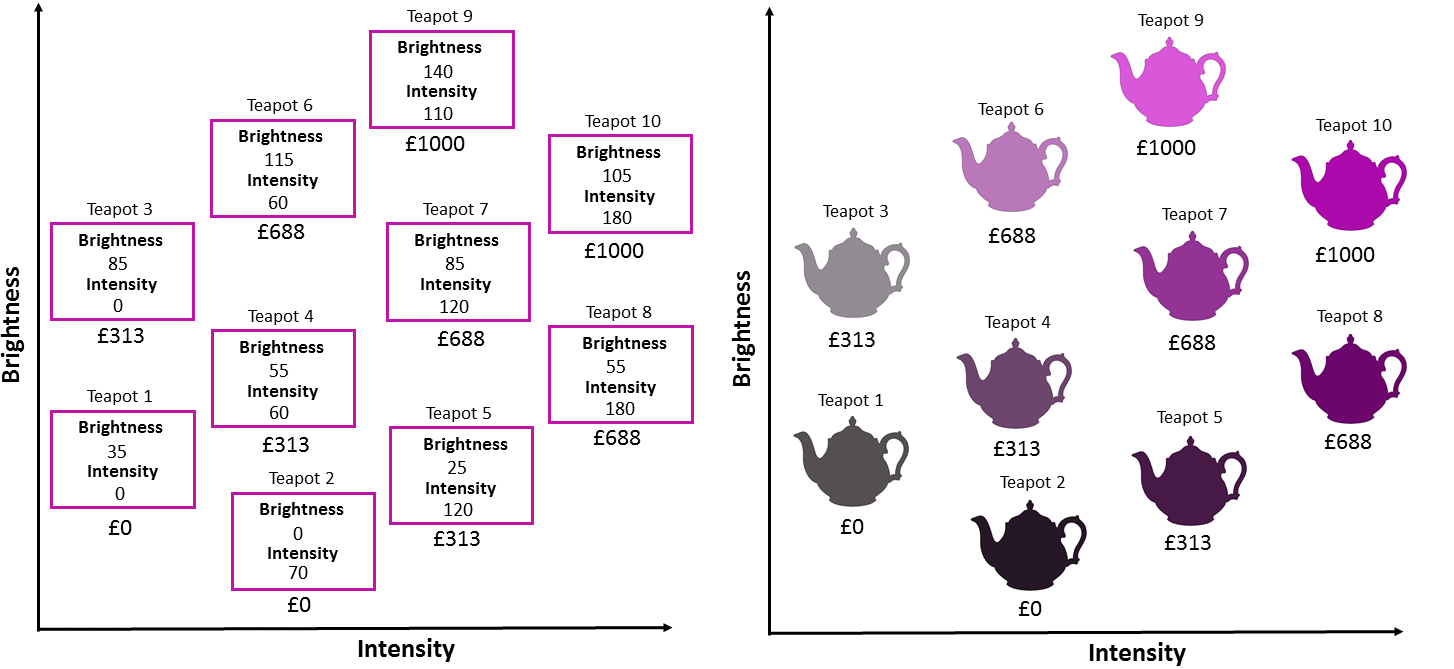
\includegraphics[width=1\textwidth]{./value_maps.png}
\label{fig:valuemaps}
\end{figure}

In the numerical condition, we invited participants to try to infer the trade-off between the two attribute dimensions before starting the learning stage. The true underlying trade-off is reflected by the red line on Figure \ref{fig:explain}: a two unit change in intensity is equal to a one unit change in brightness.

Each learning stage consisted of 20 questions, where participants had to guess the relative nominal values of the two displayed options, and use the keyboard to indicate which option was worth more than the other (left/right arrow), or whether they were equally valuable (up arrow), as shown on Figure \ref{fig:practicetrial}. Given that indifference between the target and competitor is crucial in invoking an attraction effect choice situation, we wanted to make sure that participants were able to recognise that two markedly different options can have a similar nominal value. After the keypress, participants were given feedback about whether the answer was correct, and were shown the actual nominal value of the displayed options, to facilitate learning.
In order to pass the learning stage and proceed to the subsequent choice stage, participants had to get at least 75\% of the questions right (at least 15 questions out of 20). However, participants could attempt to complete the learning stage as many times as they wished, and after every failed session they were encouraged to consult the relevant value map once more before trying again. 


\begin{figure}[htp!]
\centering
\includegraphics[width=0.65\linewidth]{./numprac22.png}
%\caption{Example practice trial in the numerical condition.}
\includegraphics[width=0.65\linewidth]{./picprac44.png}
\caption{Example practice trial in the numerical and pictorial condition.}
\label{fig:practicetrial}
\end{figure}


Using the 500 choice triplets, we created four types of questions for the learning stage, based on the value difference between the two options: equal (where the two options were of equal value), difficult (£100-£150 value difference), moderate (£150-£250 value difference), and easy (value difference higher than £250). Using the 1500 choice options generated for the 500 choice triplets, we created 400 questions for the learning stage, 100 questions for each difficulty level. Each learning stage session comprised of 20 questions, with 5 randomly chosen questions from the set of pre-generated questions for each difficulty level.


Once the participant had passed the learning stage, the choice stage began. Participants were presented with 80 choice triplets, and their task was to select the option with the highest nominal value. Out of the 80 questions, 12 were catch trials that served to gauge the attention of participants. On these trials, where there was a clearly dominating option out of the three displayed options. 

To create stimuli for the catch trials, we again used the pre-generated 1500 options that comprised the 500 choice triplets, by first choosing an option with a nominal value of at least £300, and then two inferior options that were at least worth £100 less than the first, high-value option. Using this method, we created 75 catch choice triplets overall. For each choice stage, the 12 catch trials were randomly chosen from the overall 75 triplets. The rest of the trials in the choice stage were attraction effect choice triplets, and were randomly selected from the 500 choice triplets (see Figure \ref{fig:choicetriplets}). During each trial in the learning and choice stage, the presentation order of the options was always randomised. Between the two conditions (pictorial/numerical), participants could take a break for as long as they liked.

\begin{figure}[htp!]
\centering
\caption{Example choice triplets (from left to right: DTC and DCT).}
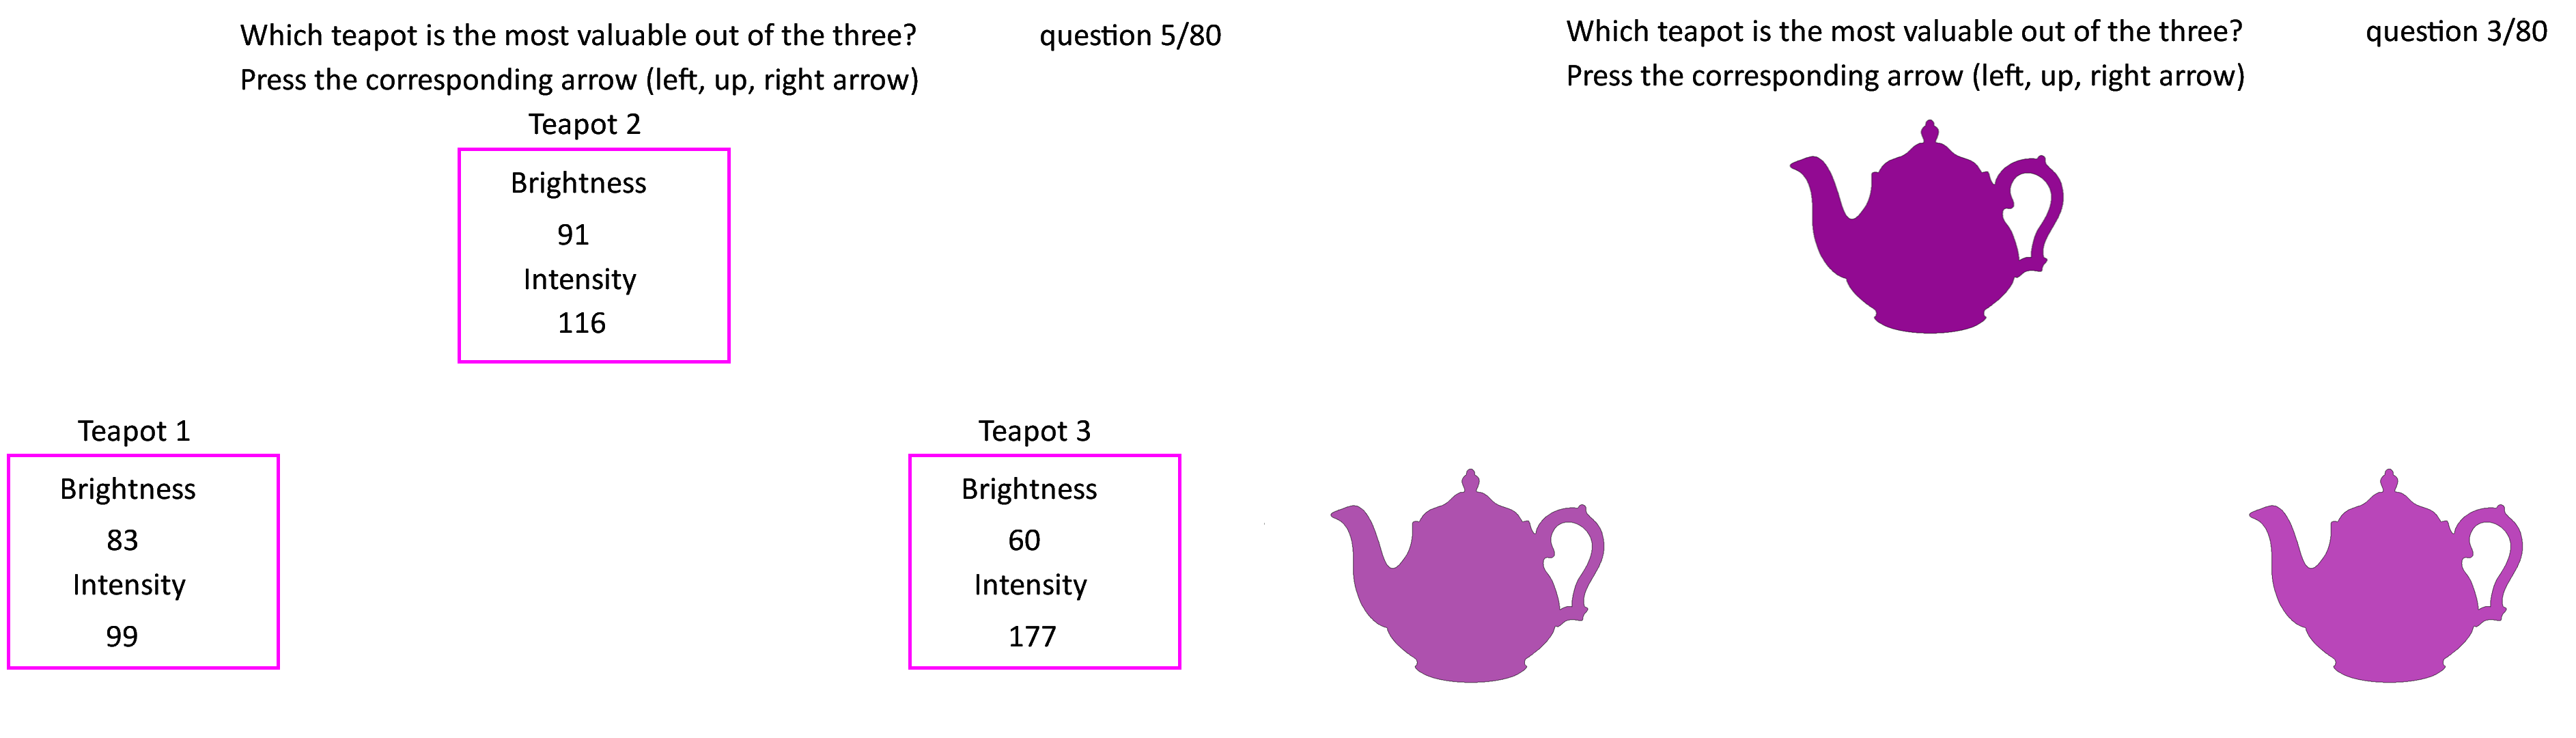
\includegraphics[width=1\textwidth]{./choice_triplets.png}
\label{fig:choicetriplets}
\end{figure}


To obtain a power level of 80\%, we calculated that a sample size of 100 will be suitable, assuming
an effect size of 0.25 (Cohen’s d). All participants were recruited through the Warwick SONA System. We obtained ethics approval from The University of Warwick’s Humanities and Social Sciences Research Ethics Committee (reference number: 50/17-18). The study was advertised as a decision-making study, and participants were given a £4 show-up fee, and were told that they could earn £0.5 for every block of 20 correct questions, therefore, the highest possible earning in this experiment was £8 (as there were 160 questions overall). Given that completing the study involved 160 choice trials (and the two practice sessions), incentive-compatibility was important to ensure that participants stayed motivated during the choice stages. The experiment automatically terminated after 50 minutes if the participant had not finished by then. 


\subsubsection{Exclusion criteria}

To ensure that we only include participants who took the task sufficiently seriously, we excluded choice blocks where the accuracy on the catch trials was 2.5 standard deviations below the average accuracy for that type of choice task (pictorial/numerical). In addition, we excluded choice blocks that fell into the lowest 2.5\% of the entropy distribution
and the upper and lower 2.5\% of the autocorrelation distribution across all participants, based on the pattern of their responses. Finally, we excluded trials that fell into the fastest 2.5\% of
the reaction time distribution, and trials where the subject selected the decoy option.
The study design, exclusion criteria and all the analyses were planned and
registered before we collected any choice data (see Appendix \ref{appchap31} for the pre-registration).

\subsection{Results}

Ideally, if all of the 100 participants had completed both conditions, we would have data from 200 choice blocks (100 pictorial and 100 numerical each). However, the learning stages had turned out to be more challenging for participants than we originally intended, and 14 people did not manage to pass the first learning stage in 50 minutes (or gave up earlier), and consequently we did not manage to collect any choice data from these participants. After applying all exclusion criteria, we were left with choice data from 86 people who completed 68 pictorial and 76 numerical choice blocks. Out of the 86 people, 61 completed both the pictorial and numeric conditions within the 50 minutes provided.

\begin{figure}
\centering
\caption{Number of practice and choice trials by condition and condition order.}
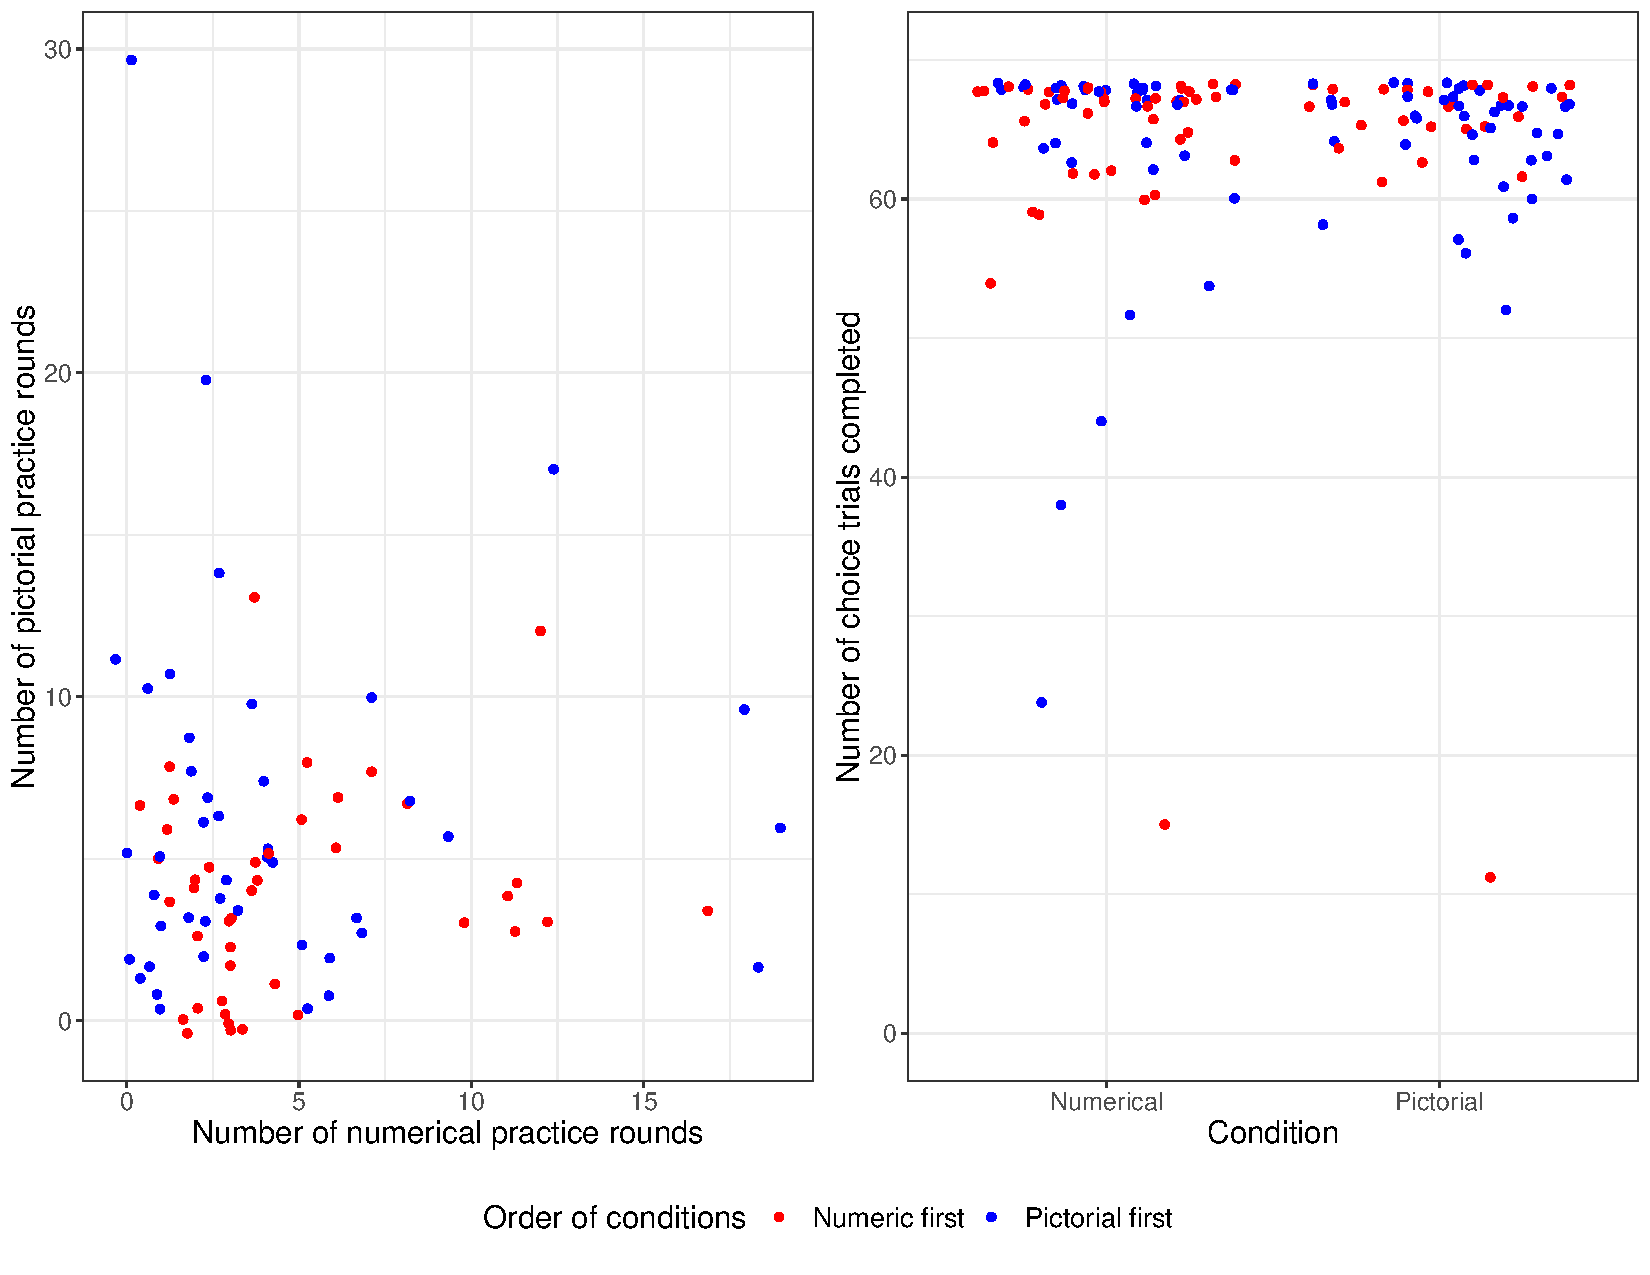
\includegraphics[width=0.9\textwidth]{./Explor_teapot.pdf}
\label{fig:Explor_teapot}
\end{figure}

The left panel on Figure \ref{fig:Explor_teapot} shows the number of attempts it took for participants to pass the numerical and pictorial learning stage (each attempt consisted of 20 questions, as explained above), by the order of the conditions (numerical/pictorial first, therefore, there are 86 dots, each of which is a participant). For the majority of participants, it took fewer than 10 attempts to pass the learning stages, and there is considerable individual heterogeneity in the number of attempts it took to complete the learning stage in the two conditions. 



The right panel in Figure \ref{fig:Explor_teapot} shows the number of completed choice trials by condition and condition order (here each dot refers to a participant's condition, there are 144 of these overall), demonstrating that the vast majority of participants have managed to finish at least one of the choice stages before the experiment was terminated. We can also see that the choice stages were more likely to be interrupted in the numerical condition than in the pictorial condition, because choice trials involving numerical choice options typically took longer.



\begin{figure}[htp]
\centering
\caption{Distribution of the proportion of trials on which the decoy was chosen by condition.}
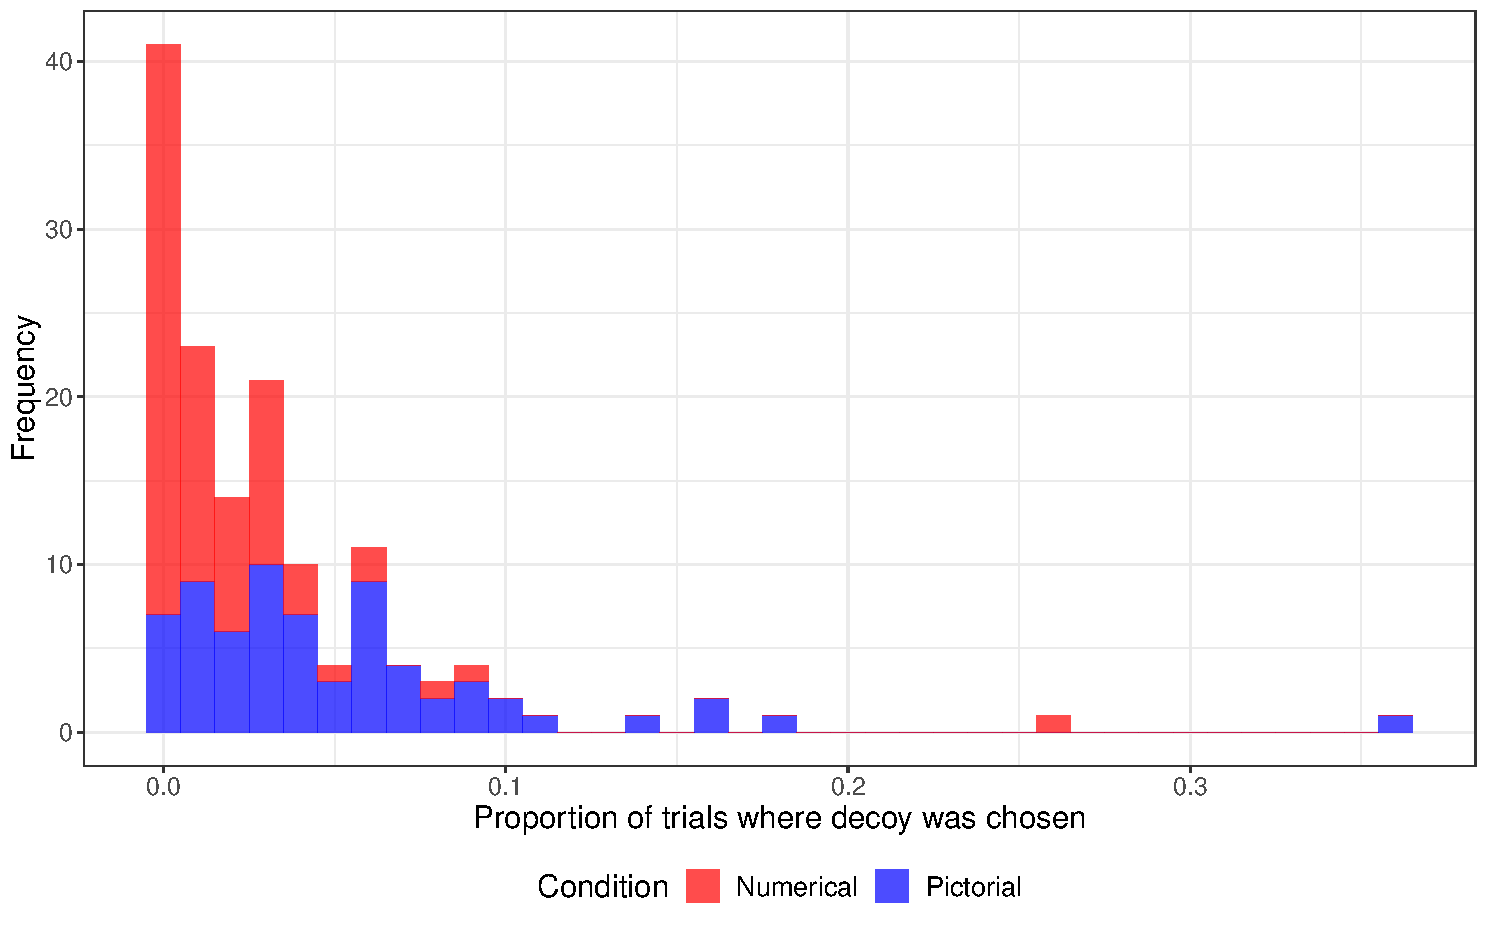
\includegraphics[width=0.8\textwidth]{./Explor_teapot_dec.pdf}
\label{fig:Explor_teapot_dec}
\end{figure}

Figure \ref{fig:Explor_teapot_dec} shows the distribution of the proportion of trials on which the decoy was chosen by condition. It can be seen that participants generally performed well in identifying dominated options (in 94\% of the 144 conditions, the proportion of the trials where the decoy was chosen was below 10\%). In addition, the decoy was never chosen in 45\% of the numerical and 10\% of the pictorial conditions, which indicates that participants found it much easier to identify the decoy in the numerical condition. This is not surprising given that in the numerical version, the choice process requires the sequential comparison of the attribute values, during which the decoy option is more likely to be identified with certainty and thus avoided, whereas in the pictorial version people are more likely to make a quicker, intuitive decision, which might result in an error. 

 To demonstrate this, Figure \ref{fig:Teapot_rts} shows the median of the reaction times (measured in seconds) scaled by subject for each subject, condition, and chosen item. As expected, participants took substantially longer to make a decision in the numerical condition. Interestingly, we do not see substantial differences in reaction times by the chosen item.

 \begin{figure}[htp]
\centering
\captionsetup{justification=centering,margin=2cm}
\caption{Distribution of the median scaled reaction times of each participant by condition and chosen item. Reaction times were first scaled by subject, then the median was calculated for each subject, condition, and chosen item. Black points and corresponding error bars represent bootstrapped 95\% CIs of the means of these medians, weighted by the number of trials.}
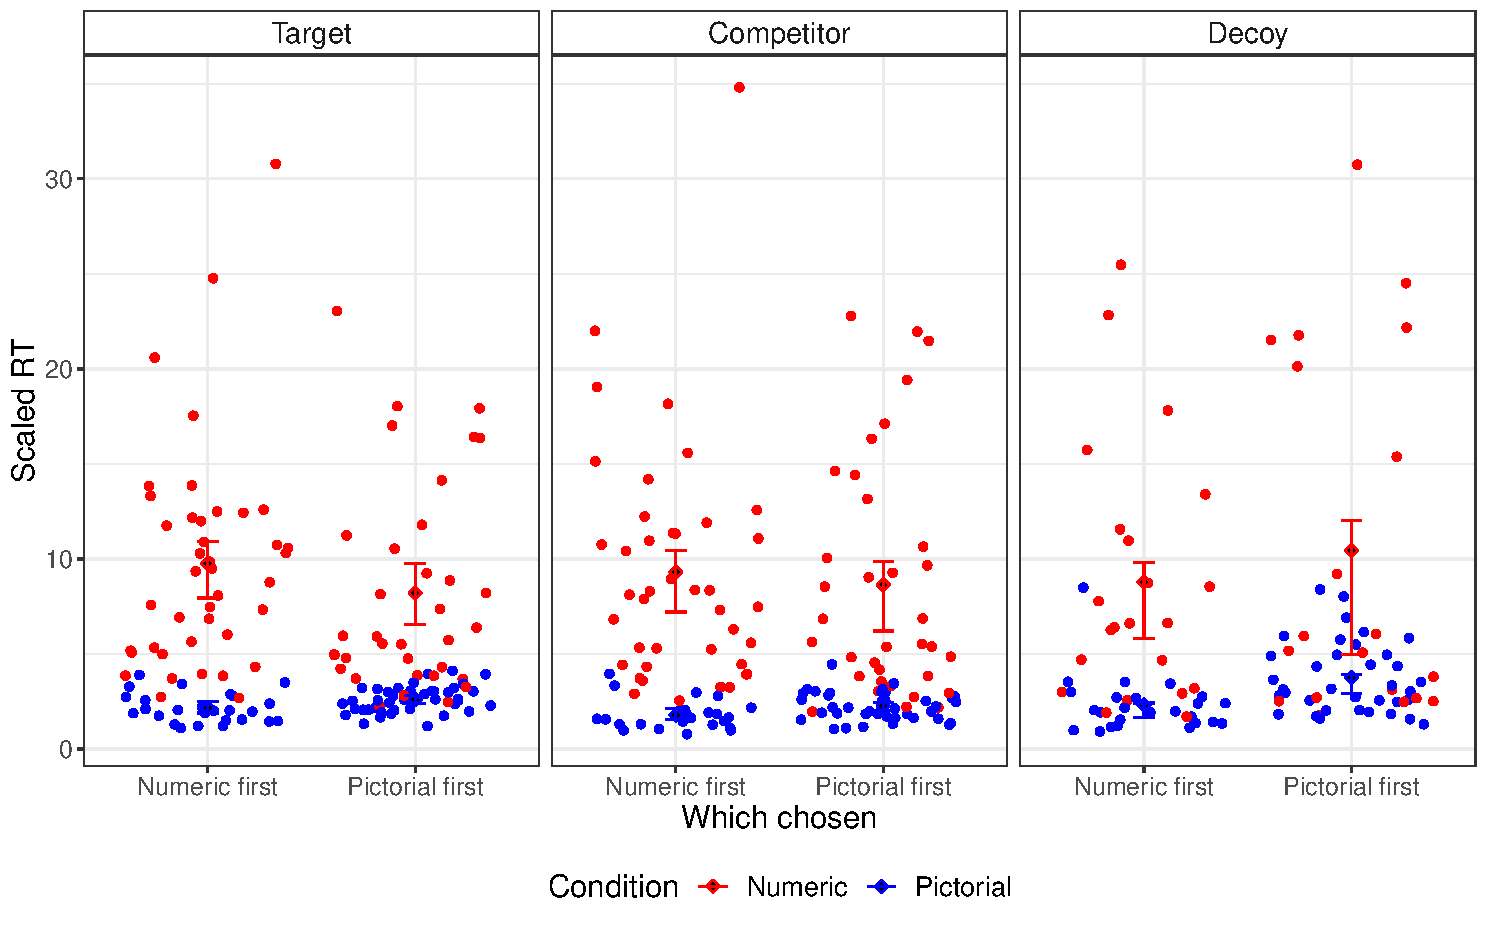
\includegraphics[width=0.9\textwidth]{./Teapot_rts.pdf}
\label{fig:Teapot_rts}
\end{figure} 


 In addition, there were no differences in the performance on the catch trials between the numerical and pictorial conditions (paired Wilcoxon Signed-Rank Test using data from the 58 participants who completed both conditions, p = .482), showing that participants were equally good at spotting a dominating option in the two types of choice tasks.

As specified in the pre-registration, to investigate how the attraction effect depends on the presentation format of the stimuli, we first tested whether the order of the conditions had any effect on the strength of the attraction effect. We did not expect presentation order to have any effect on the strength of the effect. For each participant and condition, we calculated the attraction effect as the proportion of all trials on which the target was chosen, after excluding trials where the decoy was chosen. The left panel on Figure \ref{fig:Teapot_condorder} shows the distribution of the proportion of trials on which the target was chosen. We can see that while the order of the conditions does not affect the strength of the attraction effect in the pictorial choice task, there is a pronounced increase in the tendency to choose the target in the numerical condition if it follows the pictorial choice task. The right panel of Figure \ref{fig:Teapot_condorder} echoes the same pattern, showing the strength of the effect in the two choice tasks for the subset of participants who completed both types of choice tasks (of which there were 58).   

\begin{figure}[htp]
\centering
\caption{Proportion of trials on which the decoy was chosen by condition.}
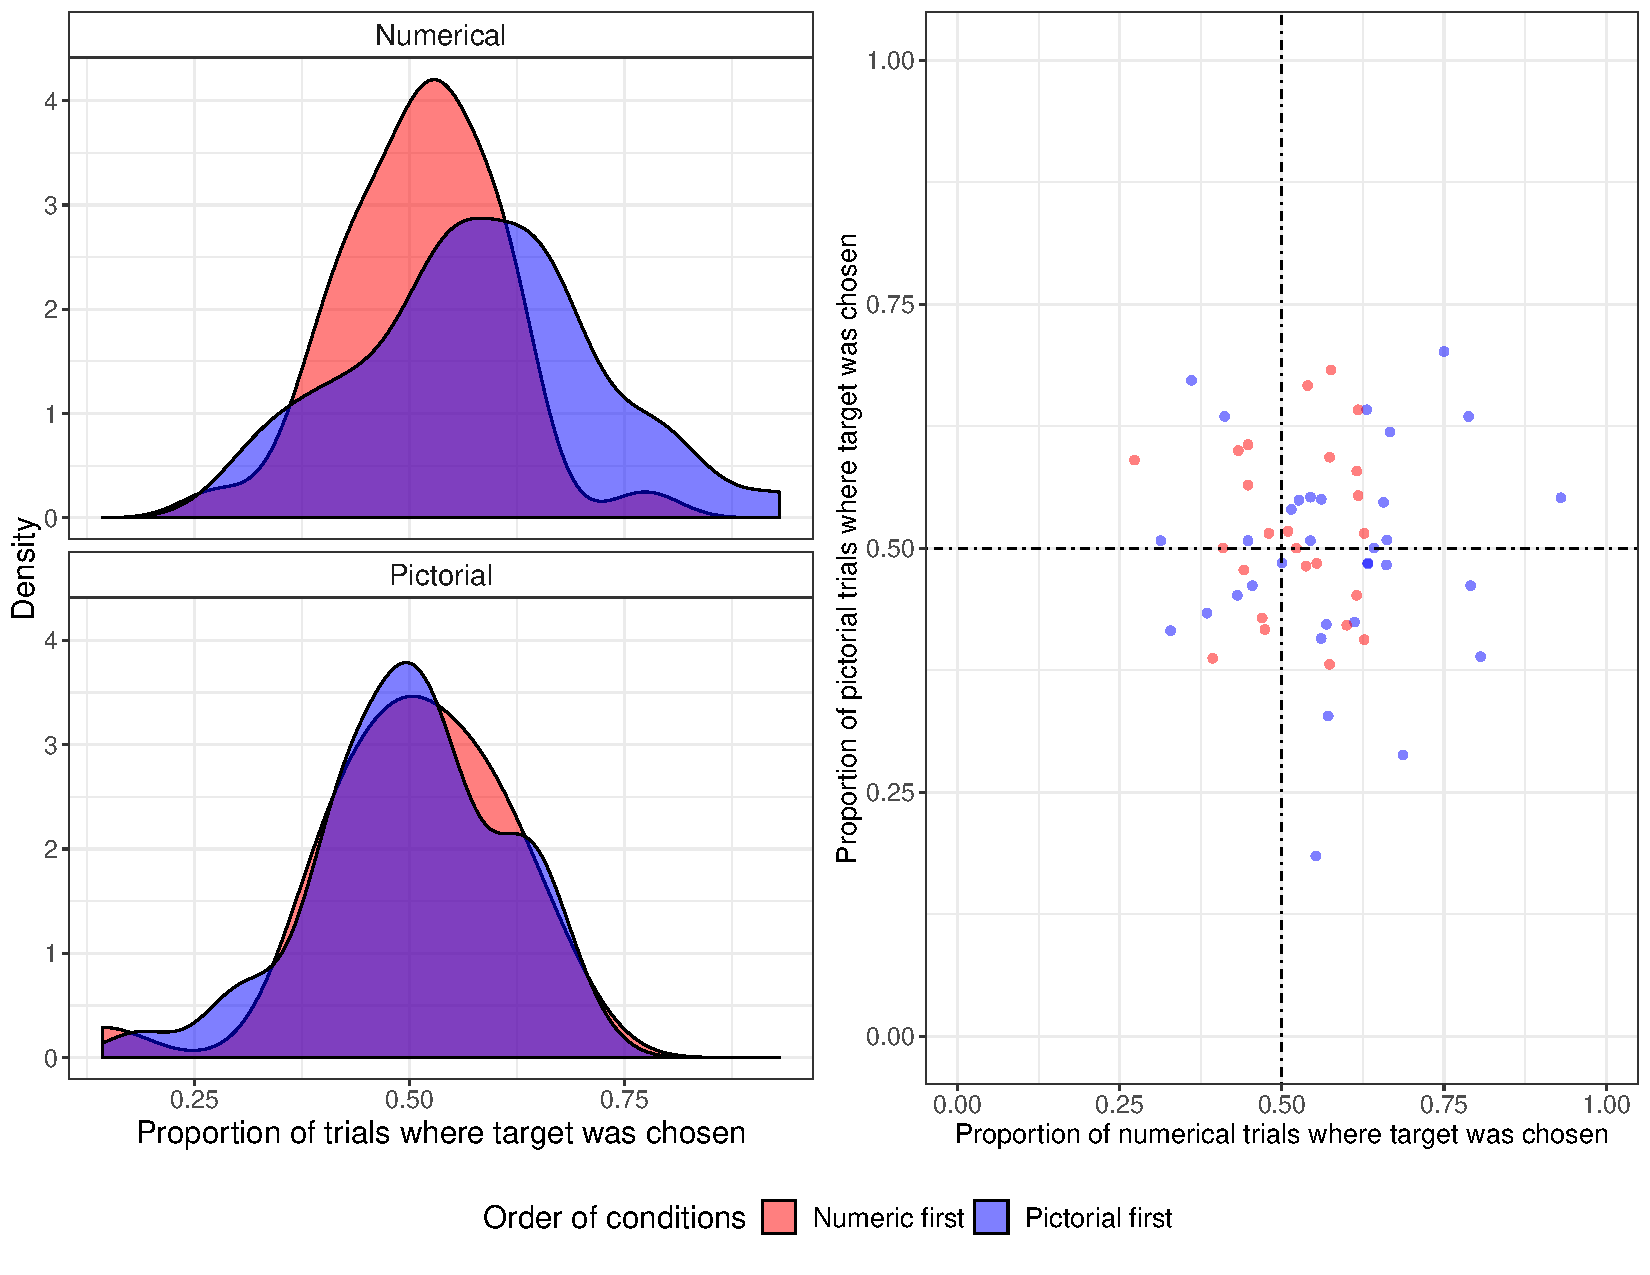
\includegraphics[width=0.8\textwidth]{./Teapot_condorder.pdf}
\label{fig:Teapot_condorder}
\end{figure}


\begin{table}[!htbp] \centering 
\captionsetup{justification=centering}
  \caption{Odds-ratios from a logistic regression (weighted by the number of trials). 95\% CIs are in brackets.} 
  \label{mixedeff} 
\begin{tabular}{@{\extracolsep{5pt}}lc} 
\\[-1.8ex]\hline 
\hline \\[-1.8ex] 
 & \multicolumn{1}{c}{\textit{Dependent variable:}} \\ 
\cline{2-2} 
\\[-1.8ex] & Target chosen proportion \\ 
\hline \\[-1.8ex] 
 Condition:Numerical & 1.001 (0.876, 1.145) \\ 
  Order:Pictorial first & 0.946 (0.789, 1.137) \\ 
  Condition:Numerical$\cdot$Order:Pictorial first & 1.405$^{***}$ (1.173, 1.684) \\ 
  Constant & 1.059 (0.919, 1.219) \\ 
 \hline \\[-1.8ex] 
Observations & 144 \\ 
Log Likelihood & $-$508.063 \\ 
Akaike Inf. Crit. & 1,026.126 \\ 
Bayesian Inf. Crit. & 1,040.975 \\ 
\hline 
\hline \\[-1.8ex] 
\textit{Note:}  & \multicolumn{1}{r}{$^{*}$p$<$0.1; $^{**}$p$<$0.05; $^{***}$p$<$0.01} \\ 
\end{tabular} 
\end{table} 


Table \ref{mixedeff} shows the results from a  mixed-effects logistic regression, where we explore how the strength of the effect varies by condition and condition order.  The results again indicate that the strength of the attraction effect in the numerical condition is much more pronounced when the first condition was pictorial. Specifically, switching the order of the two conditions (from numerical first to pictorial first) results in a 40\%, 95\% CI [17\%, 68\%], increase in the odds of choosing the target in the numerical condition. 

Since the order of the conditions unexpectedly modulated the strength of the effect effect, we only used every participant's first condition for our final test of the attraction effect, as specified in our pre-registration. As expected from the visual inspection of Figure \ref{fig:Teapot_condorder}, using Welch's t-test, we found no difference between the proportion of trials where the target was chosen in the pictorial (M = 0.5, 95\% CI [0.47\%, 0.53\%], N = 41) or numerical (M = 0.51, 95\% CI [0.49\%, 0.54\%], N = 42) condition, t(78.87) = 0.65, p = .52.

\subsection{Discussion}

To summarise, our results are somewhat mixed. On the one hand, we have not found evidence for the attraction effect in the pictorial condition, which was expected. On the other hand, we found that the strength of the attraction effect strongly depended on the order of the conditions in the numerical condition, with a markedly higher likelihood of the target being chosen if the numerical condition followed the pictorial condition. 

This was unexpected, as we predicted to see the attraction effect in the numerical condition, regardless of the order of the conditions. This surprised us, for two reasons. First, decades of decision-making research suggests that the attraction effect is a reliable phenomenon when attribute values are displayed numerically, but participants were indifferent between the target and competitor when the numerical condition came first. In addition, it is not immediately obvious why the order of the conditions would have such a strong effect on the susceptibility to the attraction effect. We can only speculate about the reasons behind these puzzling results.

One obvious difference between our experimental task and the standard attraction effect choice paradigm is that in our task, participants had to learn the underlying trade-off between the attribute values, as opposed to relying on a more intuitive, preferential valuation rule. This is problematic for two reasons. First, it might mean that our artificial valuation rule was conceptually different from a standard preferential choice task (where valuation is more intuitive), as the choice process involved consulting a previously learnt rule, which is unlikely to resemble a preferential choice process. A second, related issue is that in the practice stages, we trained participants to be experts in inferring the nominal value of the options, while it has been previously shown that the attraction effect tends to be stronger when the decision maker is unfamiliar with the choice domain, and weakens with expertise (e.g., \citeNP{Huber2014}). This is supported by the fact that increasing the number of practice trials slightly reduces the attraction effect, as one additional practice trial decreases the odds of choosing the target by 5.8\%, 95\% CI [3\%, 10.9\%] (see regression results in Appendix \ref{appchap32}).

However, even if these concerns have some validity, they do not offer a comprehensive explanation for our results. Specifically, they cannot accommodate the fact that we found a strong effect of condition order. Our results show a strong attraction effect in the numerical condition when it follows the pictorial condition, and no attraction effect when the numerical condition comes first. 

One explanation for such a strong temporal effect could be that cognitive fatigue affected participants' decision making in the second half of the experiment. As mentioned before, the learning stages of the experiment proved to be much harder than we expected and intended, illustrated by the fact that 42\% of the participants did not manage to complete the experiment within 50 minutes, with 14 people giving up altogether before passing the first learning stage. In addition, the numerical condition required significantly more cognitive effort than the pictorial task, reflected by the much longer reaction times (see Figure \ref{fig:Teapot_rts}). 

It has been previously suggested that depletion of cognitive resources (induced by a Stroop-task that preceded the choice stage) results in a more pronounced attraction effect due to higher reliance on intuitive decision processes \cite{Pocheptsova2009a}. This conclusion is supported by the finding that the attraction effect is stronger for those who are more likely to engage in intuitive reasoning \cite{Mao2012}, although a later replication attempt failed to reproduce the same choice pattern for depleted participants \cite{DeHaan2015}.  
The link between cognitive fatigue and susceptibility to the attraction effect remains ambiguous in the literature, and we cannot test the role of cognitive fatigue in the context of our choice experiment, as we did not measure fatigue. In addition, the slight negative effect of the number of practice trials on the strength of the attraction effect is not consistent with a fatigue-based explanation.

Previous research has suggested that the attraction effect strengthens when deliberation time increases \cite{Trueblood2014}, although cognitive fatigue, if present, is likely to alter this relationship. While Figure \ref{fig:Teapot_rts} shows a very slight tendency towards shorter reaction times when the target is chosen in the numerical condition when it follows the pictorial condition, this difference is not statistically significant (Wilcoxon Signed-Rank Test using data from the 58 participants who completed both conditions, p = .864).

If participants got tired towards the end of the experiment, \textit{and} they are more susceptible to the attraction effect in the numerical condition after a prolonged period of cognitive effort, then we would expect that the likelihood of choosing the target increases throughout the choice stage. To test this hypothesis, we explored how the tendency to choose the target changed over time within a condition (numerical/pictorial), depending on the order of the conditions.

To this end, we divided the number of trials in each condition into 4 equal sized blocks (in their temporal order), and calculated the corresponding target choice proportions for each blocks. If the overall number of trials were not a multiple of 4, then the remainder was allocated to the fourth block. 

Figure \ref{fig:Block_order} shows the average proportion of trials where the target was chosen by condition, condition order and block number, revealing a slightly increasing temporal tendency to choose the target in the numerical condition if it follows the pictorial condition. Interestingly, the pattern is absent from all other condition-order combinations. While it is likely that our findings are a result of a complex interplay between several factors that we did not predict when we designed the experiment, cognitive fatigue seems to be an appropriate candidate theory for explaining the strong link between the strength of the attraction effect in the numerical condition and condition order in our experiment.


\begin{figure}
\centering
\caption{Mean target choice share by condition, condition order and block number. Error bars represent 95\% bootstrapped CIs, weighted by the number of trials in each block.}
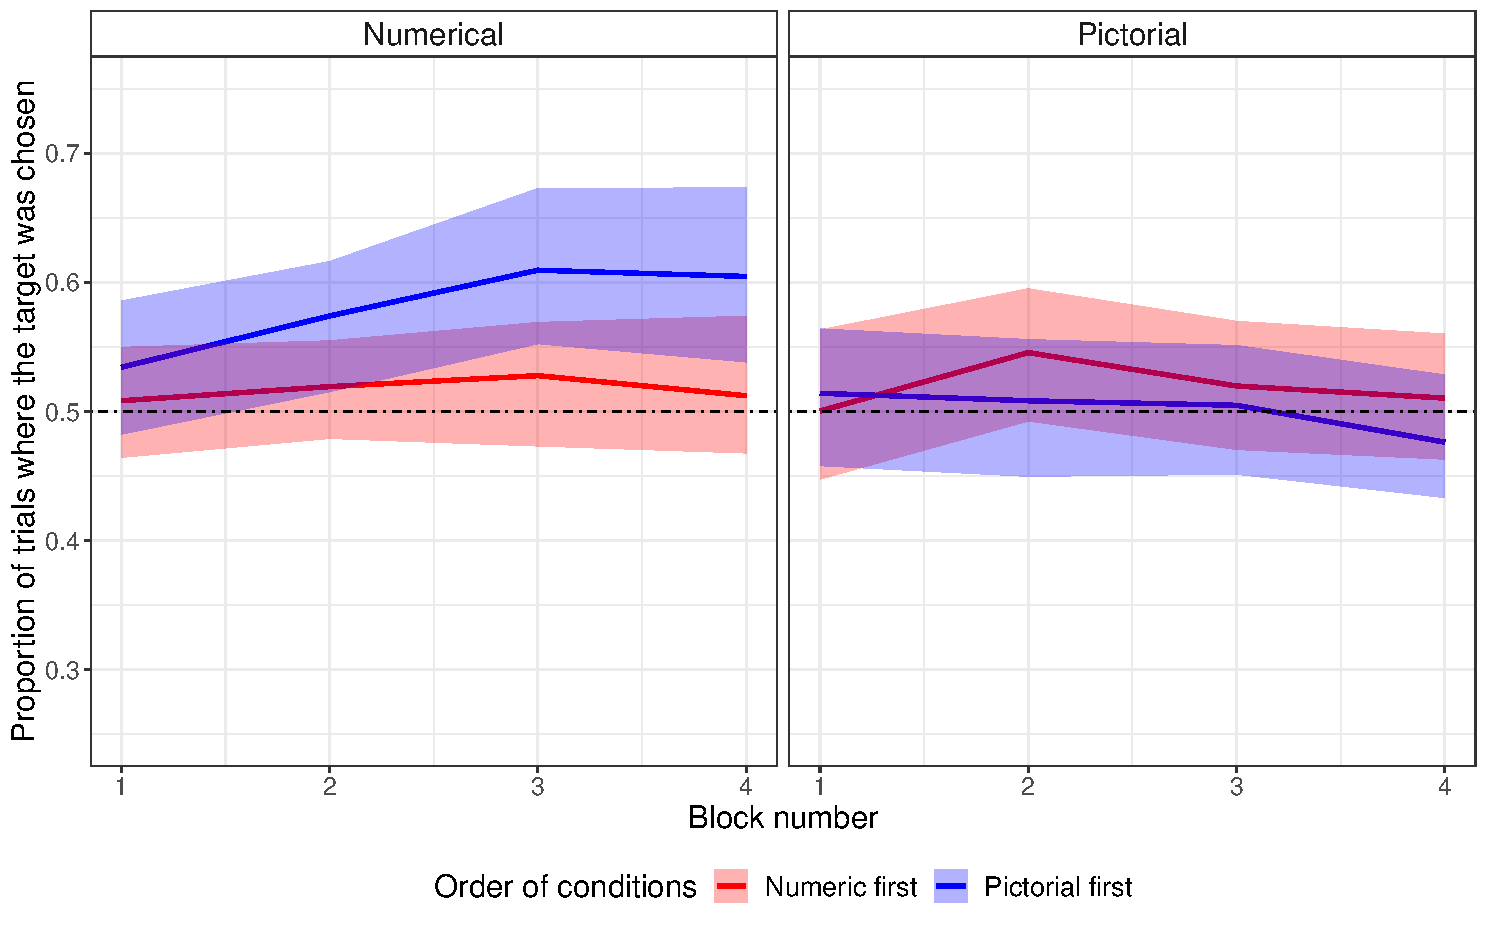
\includegraphics[width=1\textwidth]{./Block_order.pdf}
\label{fig:Block_order}
\end{figure}


\section{General Discussion}

This study set out to investigate how the attraction effect depends on the presentation format of the stimuli. Our earlier study described in Chapter \ref{AE_LSA} had failed to replicate the effect using a complex, naturalistic stimuli. We hypothesized that stimuli presentation, and more specifically, the possibility of serial processing of the attribute dimensions might be key in explaining the seemingly elusive nature of this decision bias.

Using insights from decades of psychological research on information processing, we  created a simplified, artificial stimuli that can be represented in a pictorial and numerical format, to test if it is the separable nature of the attribute dimensions that gives rise to the attraction effect.  We expected to see a strong attraction effect in the numerical condition, and no attraction effect in the pictorial condition.

Somewhat unexpectedly, we found a strong attraction effect in the numerical condition, but only when it followed the pictorial condition. The likelihood of choosing the target showed an upward temporal trend in this numerical condition, consistent with a cognitive fatigue explanation, but our data did not allow us to to directly test the link between cognitive fatigue and susceptibility to the attraction effect.

While we cannot offer a comprehensive explanation for these contradictory results, we also recognise that artificially induced preferences (created by our imposed valuation rule) are unlikely to give rise to the same decision processes as more  intrinsic preferences, where little or no cognitive effort is required to make a decision. For this reason, we suggest that any test of the attraction effect using perceptual stimuli should aim to use a simple rule to guide choices, as these are more likely to resemble real-life preferential decisions, and thus are better suited to probe the attraction effect under different stimuli formats. 

A more comprehensive investigation of how the strength of the attraction effect depends on the stimuli presentation format could explore how the separability of the attribute dimensions alter this relationship. For example, a purely numerical condition could be compared to a perceptual version, with spatially separable attribute dimensions (e.g., width and height of rectangles, \citeNP{Trueblood2013}). Then, in another condition, the presentation of the pictorial stimuli could be spatially non-separable, preventing the serial processing of the attribute dimensions. The final condition could test the strength of the effect with integral dimensions (e.g., intensity and brightness), but with no imposed valuation rule. Differences in the strength of the attraction effect between these conditions could provide us with important insights about the cognitive processes underlying this decision bias.


\bibliographystyle{apacite}

\newpage

\bibliography{refs}


\section{Appendix}

 \begin{figure}[H]
    \captionsetup{justification=centering}
\centering
\caption{Pre-registration of Experiment 1 from Chapter \ref{AE_Teapots}.}

\includegraphics[width=1\textwidth]{AE_Teapot_aspred.pdf}
\end{figure}

\newpage
 \label{appchap32} 
  
  \begin{table}[!htbp] \centering 
\captionsetup{justification=centering}
  \caption{Odds-ratios and 95\% CIs from a mixed-effects logistic model with subject-specific intercepts, Experiment 2. (T - Target, C - Competitor, D - Decoy)} 
  \label{latentattr_exp2reg} 
\resizebox{10cm}{!}{\begin{tabular}{@{\extracolsep{5pt}}lc} 
\\[-1.8ex]\hline 
\hline \\[-1.8ex] 
 & \multicolumn{1}{c}{\textit{Dependent variable:}} \\ 
\cline{2-2} 
\\[-1.8ex] & Target chosen proportion \\ 
\hline \\[-1.8ex] 
 Condition:Numerical & 1.028 (0.897, 1.179) \\ 
  Order:Pictorial first & 0.974 (0.811, 1.172) \\ 
  Practice attempts & 0.942$^{**}$ (0.891, 0.997) \\ 
  Condition:NumericalXOrder:Pictorial first & 1.351$^{***}$ (1.124, 1.625) \\ 
  Constant & 1.038 (0.900, 1.195) \\ 
 \hline \\[-1.8ex] 
Observations & 144 \\ 
Log Likelihood & $-$505.947 \\ 
Akaike Inf. Crit. & 1,023.895 \\ 
Bayesian Inf. Crit. & 1,041.713 \\ 
\hline 
\hline \\[-1.8ex] 
\textit{Note:}  & \multicolumn{1}{r}{$^{*}$p$<$0.1; $^{**}$p$<$0.05; $^{***}$p$<$0.01} \\ 
\end{tabular} }
\end{table}


\end{document}